\section*{Introduction}
Soit une poutre de section carré et de longueur "infinie" soumise à une charge $F$ sur sa moitié centrale supérieur. On se propose d'étudier la résistance de cette poutre lorsqu'elle est chargée verticalement. On définie le champs de contraintes $\sigma = \begin{pmatrix}
\sigma_{xx} & \sigma_{xy}\\
\sigma_{xy} & \sigma_{yy}
\end{pmatrix}$. On souhaite maximiser la charge imposée (c'est à dire l'intégrale de $\sigma_{yy}$ sur la surface supérieur de la poutre) sans qu'il y ait déformation plastique, sous les contraintes mécaniques suivantes : 
\begin{align}
\frac{\partial \sigma_{xx}}{\partial x} + \frac{\partial \sigma_{xy}}{\partial y} &= 0 \label{eq:contrainteequilibre1}\\
\frac{\partial \sigma_{xy}}{\partial x} + \frac{\partial \sigma_{yy}}{\partial y} &= 0\label{eq:contrainteequilibre2}\\
\sigma^{(i)}n &= \sigma^{(j)}n & \text{si le triangles $(i)$ et $(j)$ ont un côté de normale $n$ en commun} \label{eq:contrainteContinuite}\\
\sigma n &= 0 & \text{sur les frontières latérales} \label{eq:contrainteFrontiere} \\
(\sigma_{xx} - \sigma_{yy})^2 + (2 \sigma_{xy})^2 & \leq 4 k^2 \label{eq:contrainteTresca}\\
\end{align}
où les contraintes \eqref{eq:contrainteequilibre1} et \eqref{eq:contrainteequilibre2} expriment la conservation de la quantité de mouvement; et la contrainte \eqref{eq:contrainteTresca} est le critère de plasticité de Tresca-von Mises. 


Comme ce problème possède une infinité de contraintes (problème continu), nous le discrétisons en triangles comme à la figure \ref{fig:discretisation}. Un nœud peut prendre plusieurs valeurs $\sigma$ si il appartient à plusieurs triangles. 

\begin{figure}[h!]
\centering
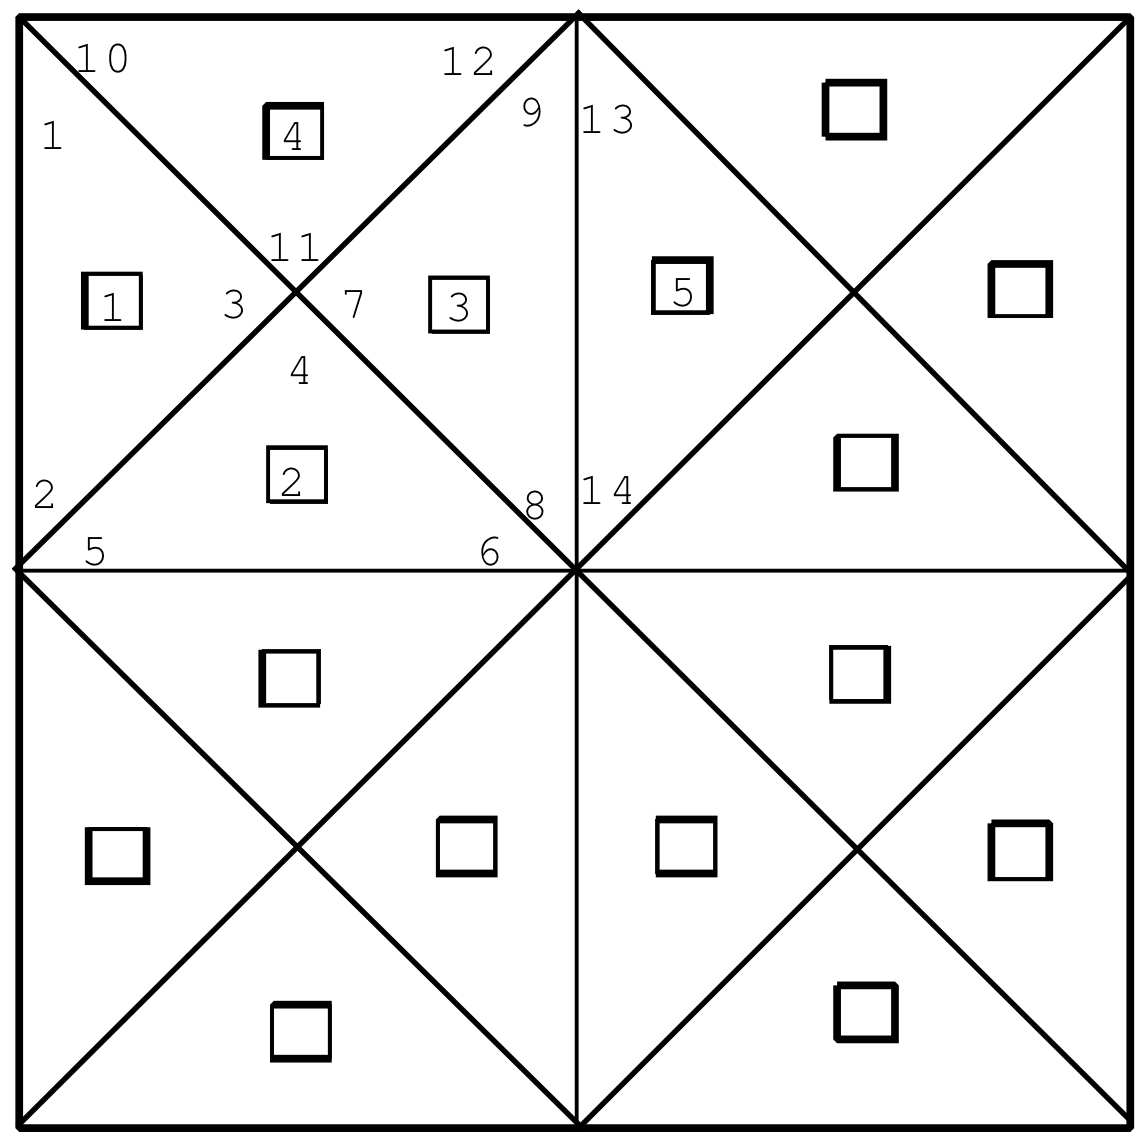
\includegraphics[height=5cm]{images/discretisation.png}
\caption{Section de la poutre discrétisée en triangles}
\label{fig:discretisation}
\end{figure}


\newpage
\section{Modélisation}
Soit $L$ la longueur d'un côté de la poutre. On défini $l=\frac{L}{N}$, la longueur d'un côté d'un carré et $h=\frac{l}{2}$, la longueur de la hauteur d'un triangle. On considère quatre cas de triangles : 
\begin{itemize}
\item cas triangle 1, orienté comme le 1 sur la figure \ref{fig:discretisation};
\item cas triangle 2, orienté comme le 2 sur la figure \ref{fig:discretisation};
\item cas triangle 3, orienté comme le 3 sur la figure \ref{fig:discretisation};
\item cas triangle 4, orienté comme le 4 sur la figure \ref{fig:discretisation};
\end{itemize} 
et dans chacun des cas, on écrit les conditions de divergence nulle comme des différences finies. 


Pour les conditions de continuité, on distingue également quatre cas : 
\begin{equation}
\overrightarrow{n} = \begin{pmatrix}
1\\
-1
\end{pmatrix}, 
\overrightarrow{n} = \begin{pmatrix}
1\\
1
\end{pmatrix}, 
\overrightarrow{n} = \begin{pmatrix}
1\\
0
\end{pmatrix},
\overrightarrow{n} = \begin{pmatrix}
0\\
1
\end{pmatrix}
\end{equation}

La fonction objectif correspond à une règle des trapèze sur les $\sigma_{yy}$ des triangles en lesquels le bloc exerce la force (appelons cet ensemble $\mathcal{F}$; il s'agit de triangles de type 4. Nous appelons les sommets supérieur de ce triangles 1 et 3). Cela donne
\begin{align*}
\max \sum_{i \in \mathcal{F}} L \frac{\sigma_{yy}^1 + \sigma_{yy}^3}{2}
\end{align*}

Les conditions de continuité donnent, en nommant $a,b$ les points d'un coté du segment et $c,d$ les points de l'autre coté : \\
\begin{center}
\begin{minipage}{0.4\textwidth}
\textbf{cas 1 : }
\begin{align*}
\sigma_{xx}^a - \sigma_{xy}^a &= \sigma_{xx}^c - \sigma_{xy}^c \\
 \sigma_{xy}^a - \sigma_{yy}^a &= \sigma_{xy}^c - \sigma_{yy}^c \\
 \sigma_{xx}^b - \sigma_{xy}^b &= \sigma_{xx}^d - \sigma_{xy}^d \\
 \sigma_{xy}^b - \sigma_{yy}^b &= \sigma_{xy}^d - \sigma_{yy}^d \\
\end{align*}
\end{minipage}
\vline
\begin{minipage}{0.4\textwidth}
\textbf{cas 2 :}
\begin{align*}
\sigma_{xx}^a + \sigma_{xy}^a &= \sigma_{xx}^c + \sigma_{xy}^c \\
 \sigma_{xy}^a + \sigma_{yy}^a &= \sigma_{xy}^c + \sigma_{yy}^c \\
 \sigma_{xx}^b +\sigma_{xy}^b &= \sigma_{xx}^d + \sigma_{xy}^d \\
 \sigma_{xy}^b + \sigma_{yy}^b &= \sigma_{xy}^d + \sigma_{yy}^d \\
\end{align*}
\end{minipage}

\begin{minipage}{0.4\textwidth}
\textbf{cas 3 :}
\begin{align*}
\sigma_{xx}^a &= \sigma_{xx}^c \\
 \sigma_{xy}^a  &= \sigma_{xy}^c \\
 \sigma_{xx}^b&= \sigma_{xx}^d\\
 \sigma_{xy}^b &= \sigma_{xy}^d  \\
\end{align*}
\end{minipage}
\vline
\begin{minipage}{0.4\textwidth}
\textbf{cas 4 :}
\begin{align*}
\sigma_{xy}^a &= \sigma_{xy}^c \\
\sigma_{yy}^a &=  \sigma_{yy}^c \\
\sigma_{xy}^b &= \sigma_{xy}^d \\
\sigma_{yy}^b &= \sigma_{yy}^d \\
\end{align*}
\end{minipage}
\end{center}

Les conditions d'équilibre donnent : 
\begin{align*}
\frac{\sigma_{xx}^3 - \frac{\sigma_{xx}^1+\sigma_{xx}^2}{2}}{h} + \frac{\sigma_{xy}^1-\sigma_{xy}^2}{l}&=0 & \text{pour triangle type 1}\\
\frac{\sigma_{xy}^3 - \frac{\sigma_{xy}^1+\sigma_{xy}^2}{2}}{h} + \frac{\sigma_{yy}^1-\sigma_{yy}^2}{l}&=0& \text{pour triangle type 1}\\
\frac{\sigma_{xx}^3-\sigma_{xx}^2}{l} + \frac{\sigma_{xy}^1 - \frac{\sigma_{xy}^3+\sigma_{xy}^2}{2}}{h} &=0& \text{pour triangle type 2}\\
\frac{\sigma_{xy}^3-\sigma_{xy}^2}{l} + \frac{\sigma_{yy}^1 - \frac{\sigma_{yy}^3+\sigma_{yy}^2}{2}}{h} &=0 & \text{pour triangle type 2}\\
\frac{\frac{\sigma_{xx}^3+\sigma_{xx}^2}{2} - \sigma_{xx}^1 }{h} + \frac{\sigma_{xy}^3-\sigma_{xy}^2}{l}&=0& \text{pour triangle type 3}\\
\frac{\frac{\sigma_{xy}^3+\sigma_{xy}^2}{2} - \sigma_{xy}^1 }{h} + \frac{\sigma_{yy}^3-\sigma_{yy}^2}{l}&=0& \text{pour triangle type 3}\\
\frac{\sigma_{xx}^3-\sigma_{xx}^1}{l} + \frac{\frac{\sigma_{xy}^1+\sigma_{xy}^3}{2} - \sigma_{xy}^2 }{h} &=0 & \text{pour triangle type 4}\\
\frac{\sigma_{xy}^3-\sigma_{xy}^1}{l} + \frac{\frac{\sigma_{yy}^1+\sigma_{yy}^3}{2} - \sigma_{yy}^2 }{h} &=0 & \text{pour triangle type 4}\\
\end{align*}


Les conditions frontières donnent, pour tout nœud $a$ appartenant à une frontière latérale : 
\begin{align*}
\sigma_{xx}^a&= 0\\
 \sigma_{xy}^a &= 0  \\
\end{align*}

Les conditions frontières donnent, pour tout nœud $a$ appartenant au premier quart ou au dernier quart de la frontière supérieur (en fait c'est un peu plus subtil que ça, comme $N$ n'est pas toujours un multiple de 4, on a $2\lfloor \frac{N}{4} \rfloor + 1 \left( \lceil \frac{N}{4} \rceil - \lfloor \frac{N}{4} \rfloor \right) = \lfloor \frac{N}{4} \rfloor + \lceil \frac{N}{4} \rceil$ points en lesquels il faut imposer une contrainte de chaque côté du bloc exerçant la force; c'est-à-dire au total $4*\left(  \lfloor \frac{N}{4} \rfloor + \lceil \frac{N}{4} \rceil \right)$ contraintes) : 
\begin{align*}
\sigma_{yy}^a&= 0\\
 \sigma_{xy}^a &= 0  \\
\end{align*}
Toutes les contraintes énoncée précédemment forment un système $Ax=b$. A cela viennent s'ajouter les contraintes de von Mises qui sont convexes. Notre problème d'optimisation est donc convexe et s'écrit 
\begin{align*}
& \max c^T x\\
 Ax &= b\\
 x \in \mathcal{X}
\end{align*}
où $\mathcal{X}$ est l'ensemble décrit par les contraintes de von Mises. L'appartenance à cet ensemble sera imposer au moyens de fonctions barrières (voir méthodes des point intérieur). 


Si $N$ est le nombre de carrés sur un côté de la section de la poutre, alors on a :
\begin{align*}
\text{\# carrés  } &= N^2\\
\text{\# triangles  } &= 4N^2\\
\text{\# points  } &= 12 N^2\\
\text{\# contraintes  } &= 24N^2+12N(N-1)+8N + 4*\left(  \lfloor \frac{N}{4} \rfloor + \lceil \frac{N}{4} \rceil \right)
\end{align*}
Pour $N=4$ par exemple, on a $520$ contraintes.
